% Walk-forward factor research: baseline deep-dive + ablation ladder.
% Build: tectonic wf_book_analysis_v2.tex   (figures expected in figures2/ and figures/)
\documentclass[11pt,a4paper]{article}

\usepackage[margin=2.6cm]{geometry}
\usepackage{graphicx}
\usepackage{booktabs}
\usepackage{float}
\usepackage{caption}
\usepackage{enumitem}
\usepackage{xcolor}
\usepackage{microtype}
\usepackage{newtxtext,newtxmath}
\usepackage[hidelinks,pdfauthor={Luca Wuerker},
            pdftitle={Evolutionary Factor Research: Baseline and Ablations}]{hyperref}

\definecolor{grey}{RGB}{96,93,84}
\captionsetup{font=small,labelfont=bf,width=.92\textwidth}
\setlist{itemsep=2pt,topsep=4pt}

\title{\bfseries Evolutionary Factor Research:\\ Baseline Results and Ablations}
\author{Luca W\"urker}
\date{August 2026}

\begin{document}
\maketitle

\begin{abstract}
\noindent All runs share one protocol on the survivorship-bias-free Nasdaq-100
point-in-time panel (2010--2026): factors are researched on data up to
mid-2021, and the five years 2021--2026 are consumed as ten six-month blocks,
each scored \emph{before} the researcher may adapt to it --- an honest
walk-forward record. Part 1 examines the full evolutionary configuration
(knowledge-graph-grounded ideation, four-objective selection, progressive data
reveal) in detail; Part 2 removes one ingredient at a time to locate where the
out-of-sample value actually comes from. All numbers are signal-level
information coefficients (IC); no position construction or costs enter.
\end{abstract}

\section{The baseline: full evolutionary configuration}

Twenty generations, eight mechanism groups derived from a knowledge graph of
1{,}723 papers, three demes per group, LLM mutation/crossover operators, and a
four-objective Pareto selection (marginal value to the book, independence,
parsimony, structural novelty). The run produced 57 factors for \$250 in LLM
cost across roughly 900 scored candidates.

\begin{figure}[H]\centering
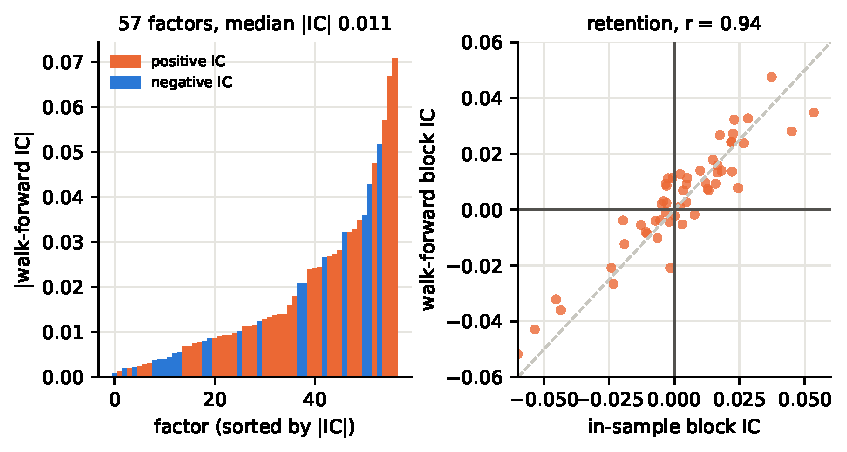
\includegraphics[width=.95\textwidth]{figures2/b1_l4_factors}
\caption{Left: the 57 surviving factors' absolute walk-forward ICs
($|$mean over the ten held-out blocks$|$ --- a stably negative factor is just
as predictive as a positive one and is sign-flipped in combination); median
$|$IC$|$ $0.011$, 65\% positive-signed. Right: in-sample versus walk-forward
signed IC per factor. Per-factor edge is essentially fully retained out of
sample ($r=0.94$; only 18\% of factors flip sign; mean $|$IC$|$ 0.019
in-sample vs.\ 0.018 walk-forward).}
\end{figure}

\begin{figure}[H]\centering
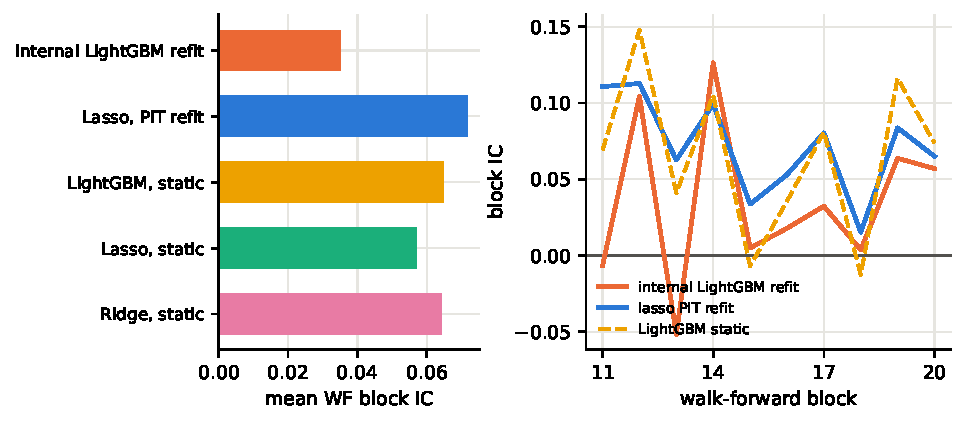
\includegraphics[width=.95\textwidth]{figures2/b2_l4_combiners}
\caption{Combining the book into one signal. The prequential LightGBM refit
the search itself uses (orange) averages $0.035$; a point-in-time lasso refit
per block reaches $0.072$ and a static ridge $0.064$ --- the factor set is
better than the score the evolution sees. The lasso is positive in every
block.}
\end{figure}

\begin{figure}[H]\centering
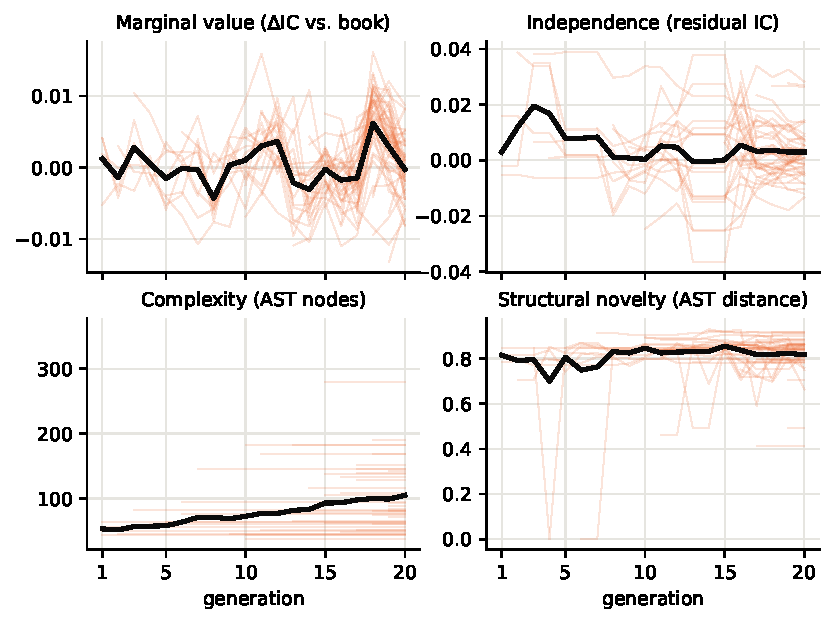
\includegraphics[width=.95\textwidth]{figures2/b3_l4_pareto}
\caption{The four selection objectives across the final archive over the
evolution (thin lines: individual factors, carried forward between re-scores;
black: archive mean). Marginal value fluctuates around zero by construction
(each survivor is measured against the rest of the book) and independence
compresses toward zero as the book fills its niches; complexity roughly
doubles over twenty generations while structural novelty stays flat at
$\sim$0.85 --- the parsimony objective slows but does not stop code growth.}
\end{figure}

\begin{figure}[H]\centering
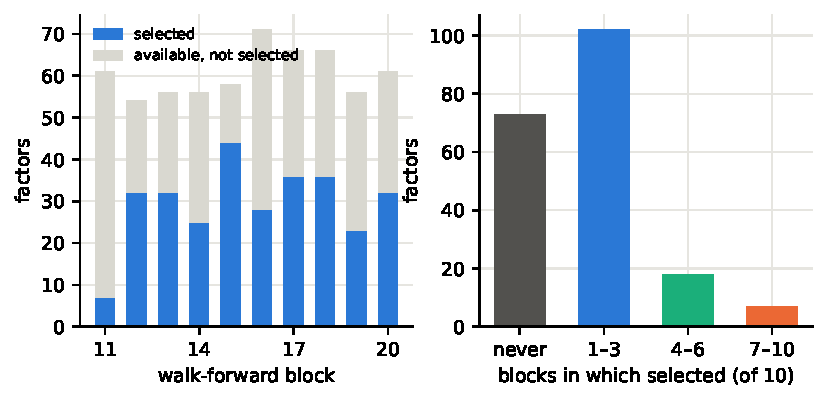
\includegraphics[width=.95\textwidth]{figures2/b4_l4_lasso}
\caption{What a sparse combiner actually uses. Per block the cross-validated
lasso keeps 7--44 of the $\sim$60 available factors (left); over the ten
refits 37\% of the $\sim$200 factors that ever entered the point-in-time pool
(archive snapshots grow through the walk-forward) are never selected and under
4\% are selected in most blocks (right) --- yet the combined IC is stable, so
the pool is redundant in a robust, interchangeable sense. Diversity confirms this: mean pairwise
$|\rho| = 0.09$, effective dimension $\approx 22$ of 57 by the
eigenvalue-participation ratio $N_{\mathrm{eff}}=(\sum\lambda_i)^2/\sum\lambda_i^2$.}
\end{figure}

\begin{figure}[H]\centering
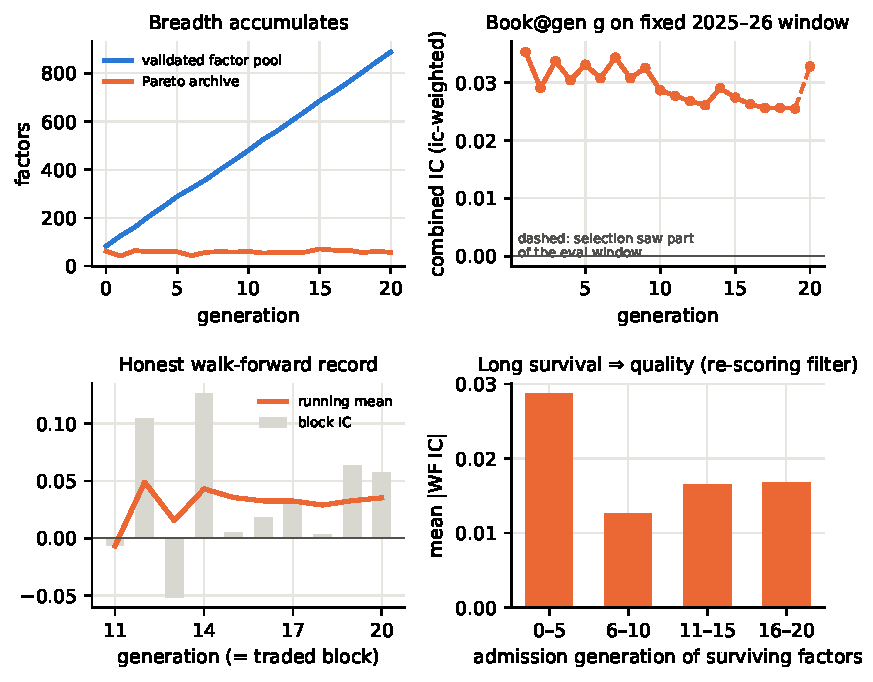
\includegraphics[width=.95\textwidth]{figures2/l3_learning}
\caption{What actually changes over the evolution (baseline arm). Top left:
the validated factor pool grows linearly (83 $\to$ 890) while the curated
archive holds at the cap --- evolution accumulates breadth. Top right: the
archive \emph{as of each generation}, recombined with identical ic-weights
fit before a fixed 2025--26 window and scored on it --- the combined IC is
flat: the generation-1 book was already as good as any later one, and
composition churn adds no combined value on untouched future data. Bottom
left: the honest prequential record accumulates and stabilises at
$\approx+0.035$ --- flatness under 20 generations of selection pressure is
the anti-overfitting machinery holding (a naive search would decay; cf.\ the
IC-only arm). Bottom right: surviving factors admitted earliest --- those
re-scored up to twenty times on growing, partially unseen windows --- have
twice the realised walk-forward $|$IC$|$ of later admits: survival through
re-scoring, not evolution's churn, is the effective quality filter.}
\end{figure}

\section{Where the value comes from: ablations}

Each arm below removes or adds one ingredient relative to the baseline,
under the identical panel, split schedule and scoring harness.

\begin{figure}[H]\centering
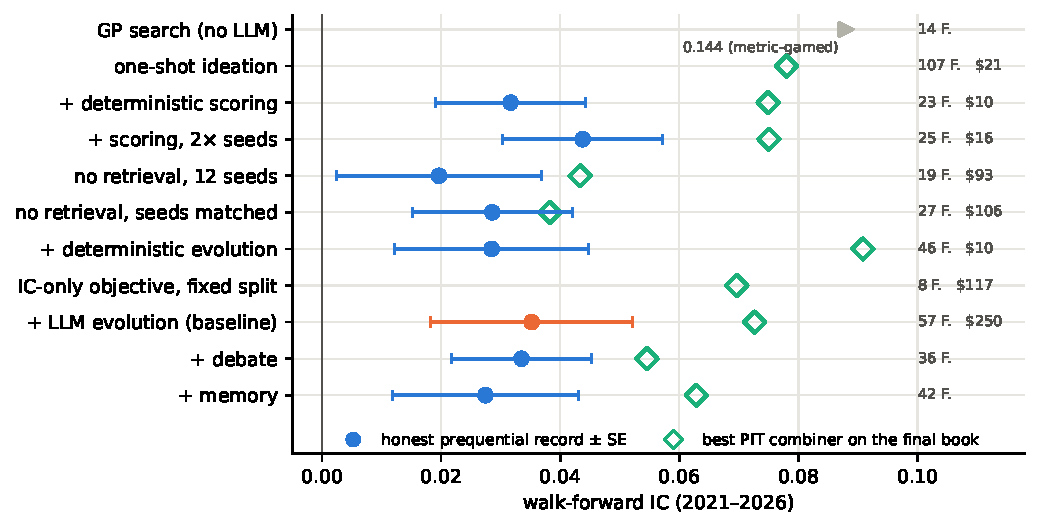
\includegraphics[width=.95\textwidth]{figures2/l1_ladder}
\caption{The ablation ladder. Filled dots: the honest prequential record
(mean of the ten block ICs $\pm$ standard error); open diamonds: the best
point-in-time combiner applied to the arm's final book; right margin: book
size and LLM cost. The GP arm's record is metric-gamed (see text) and shown
clipped.}
\end{figure}

Three readings. First, \emph{ideation plus deterministic scoring carries
almost everything}: seeding ideas once and letting the deterministic harness
score, prune and re-curate them (no evolution at all, \$10--16) lands within
block noise of the full \$250 baseline, and doubling the seed budget produced
the best honest record of the family ($+0.044$). Second, \emph{the LLM inside
the evolution adds little}: replacing all LLM mutation by deterministic
window-jitter ($+0.028$) or removing children entirely ($+0.032$) is
statistically indistinguishable from the baseline ($+0.035$, block SE
$\approx 0.012$) --- and under the best point-in-time combiner the
jitter-evolved book is in fact the family's best ($0.091$, ten of ten blocks
positive, at \$10). Third, \emph{the LLM's economic prior is what keeps the
search honest}: the prior-free GP miner ``won'' with $+0.144$ by discovering
degenerate statistics (raw price and fundamental levels whose per-underlying
IC telescopes mean reversion), and after a stationarity gate was added it
evaded the gate with near-boundary level proxies --- a Goodhart
demonstration that also explains \emph{why} the semantically grounded arms do
not overfit the same way.

Retrieval grounding needed a control to price correctly. The first two
no-retrieval runs ($+0.020$ and $+0.012$) were accidentally seeded with only
10--12 ideas instead of 96 (an oversized idea-generation call silently timed
out), confounding retrieval with seeding breadth. The seeding-matched rerun
resolves it: with 96 ungrounded ideas the no-retrieval arm reaches $+0.029$
--- statistically indistinguishable from the baseline's $+0.035$ on the
internal record --- yet its factors are individually the weakest of the
whole family (median $|$IC$|$ 0.005 vs.\ 0.011; 44\% flip sign out of
sample vs.\ 18\%; effective dimension 14 vs.\ 22, including one
near-duplicate pair), and its book recombines point-in-time to only $0.038$
versus the baseline's $0.073$. Retrieval grounding therefore does not move
the noisy headline record, but roughly doubles the deployable, combined
walk-forward IC of the resulting book. Debate and cross-run memory did not
improve on the baseline. (One mechanical caveat: in the debate arms a
sparse-coverage factor admitted early silently disabled the residual-IC
independence objective for nearly all candidates --- those two runs
effectively selected on three objectives.)

\begin{figure}[H]\centering
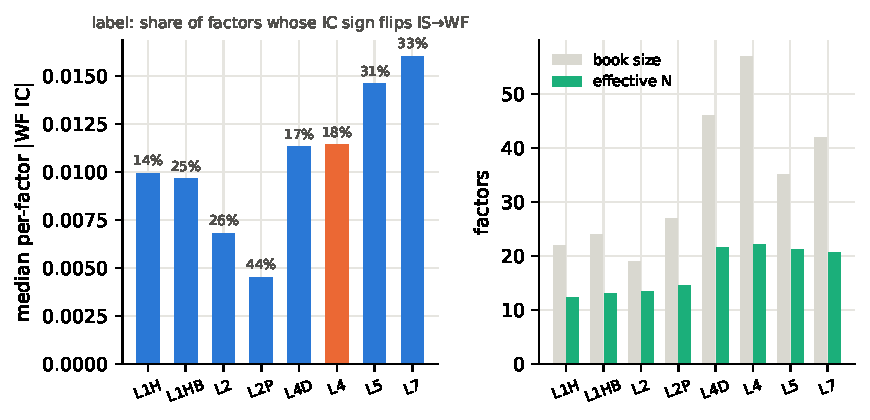
\includegraphics[width=.95\textwidth]{figures2/l2_cross_arm}
\caption{Book quality across arms (baseline in orange). Left: median
per-factor absolute walk-forward IC, with the share of factors whose IC
\emph{sign flips} from fit window to walk-forward printed above each bar.
The debate/memory books post the highest raw $|$IC$|$ medians --- but with
the worst sign stability (31--33\% flips vs.\ 18\% for the baseline), and
a quarter of their members are exact quarterly-stepped ($\rho=1.0$)
level-like signals whose per-underlying IC is mechanically inflated (9/35
and 11/42 vs.\ 4/57 in the baseline). Right: book size versus effective
independent dimension. The baseline leads where it matters for deployment:
sign stability, clean composition, breadth --- and the combined
point-in-time results.}
\end{figure}

\section{Key observations}

\begin{enumerate}
\item \textbf{The deterministic scoring harness, not the evolutionary loop,
is the workhorse.} Ideation + scoring at \$10--16 matches twenty generations
of LLM evolution at \$250 on the honest five-year record; trial counts (81
vs.\ $\sim$900) do not translate into overfitting because the anti-ratchet
machinery (progressive reveal, re-scoring, deflation) holds the record flat.
\item \textbf{Factor-level edge transfers; the combiner is the fragile
part.} Per-factor $|$IC$|$ is fully retained out of sample in every arm,
while the deployment combiner moves the headline number by a factor of two
--- report combiner-robustness, not one combiner's IC.
\item \textbf{The LLM's contribution is the economic prior at ideation.}
Removing the LLM entirely (GP) collapses into metric gaming that survives a
targeted stationarity gate; removing only retrieval grounding (seeds
matched) halves the deployable combined IC of the book ($0.038$ vs.\
$0.073$) even though the headline record barely moves.
\item \textbf{Evolution buys sign stability and breadth, not mean
performance} --- the lowest sign-flip rate, the cleanest book composition,
the largest book and highest effective dimension; relevant for downstream
combination and capacity, not for the block-mean record.
\item \textbf{The scoring design matters at the factor level, less at the
book level.} A final harness ablation (identical configuration, but
candidates scored by validation $|$IC$|$ alone on a fixed three-way split ---
no multi-objective vector, no progressive reveal; 849 candidates, \$117)
shows textbook selection overfitting per factor: the archive collapses to
one factor per mechanism group (a single-objective front is a single point),
promised validation $|$IC$|$ (median $0.040$) is cut to $0.025$ realised, and
five of the eight survivors' validation sign disagrees with their own fit
window --- selection on local noise. Yet the \emph{book} survives: eight
nearly orthogonal factors (mean $|\rho|=0.03$) recombined linearly post
strong 2021--2026 results, because the combiner re-learns the unstable signs
and the graph's group structure alone preserves diversity (its full candidate
pool, point-in-time recombined, reaches $0.070$ --- close to, but below, the
baseline's $0.073$). The multi-objective vector and progressive reveal are
what make \emph{individual factors} trustworthy; diversity structure plus a
linear combiner provide a surprising amount of insurance at the book level.
\end{enumerate}

\end{document}
